% LaTeX.tex
% Template for PROCEEDINGS PAPER of the 27th ABCM International Congress of Mechanical Engineering
% COBEM 2023
% Based on the templates of COBEM2015, COBEM2017, COBEM2019 and COBEM2021

\documentclass[10pt,fleqn,a4paper,twoside]{article}
\usepackage{abcm}
\def\shortauthor{F. Author, S. Author and T. Author (update this heading accordingly)}
\def\shorttitle{Paper Short Title (First Letters Uppercase, make sure it fits in one line)}

\begin{document}
\fphead
\hspace*{-2.5mm}\begin{tabular}{||p{\textwidth}}
\begin{center}
\vspace{-4mm}
\title{COB-2023-XXXX {\color{red}(XXXX is the identification number of the final paper)}\\
INSTRUCTIONS FOR FORMATTING THE PROCEEDINGS PAPERS OF THE 27$^{\mathrm{th}}$ COBEM}
\end{center}
\authors{First Author's Name} \\
\authors{Second Author's Name} \\
\institution{Institution and address for first and second authors - if the same} \\
\institution{e-mails} \\
\\
\authors{Third Author's Name} \\
\institution{Institution and address for third author} \\ %(If all authors are from the same institution, the "Institution and address" must be placed only once.)
\institution{e-mail} \\
\\
\authors{Same format for other authors, if any} \\
\\
\abstract{\textbf{Abstract.} The abstract should describe the objectives, context, and significance of the research, methods, results, and main conclusions of the paper in about 200 words. It should not include formulas or references to a bibliography. It must be written in only one paragraph.}\\
\\
\keywords{\textbf{Keywords:} keyword 1, keyword 2, keyword 3, \dots{}. (up to 5 keywords separated by commas)}\\
\end{tabular}

\section{INTRODUCTION}

These instructions are intended to serve as a guide for the formatting of papers to be published in the Proceedings. The proceedings of the 27$^\mathrm{th}$ COBEM will be published in Adobe\textsuperscript{TM} PDF format.

Papers MUST be formatted according to these instructions. This file can be used as a template for LaTeX. LaTeX is available as free software. It can also be used as a formatting guide for users of other word processing programs.

Submissions are limited to a minimum of 6 pages and a maximum of 10 pages, including tables and figures. 

\section{TEXT FORMAT}

Manuscripts should be in English, typewritten on A4 pages in Times New Roman font, size 10, except for the title, author affiliation, abstract, and keywords, for which special formatting instructions are given above. Use single space between lines throughout the text.

The block of text containing the title, author names and affiliations, abstract, and keywords must be indented 0.1 cm from the left margin and marked by a $2\ 1/4$ pt wide black line on the far left.

Pages must have a top margin of 3 cm and all other margins (left, right, and bottom) must have 2 cm. The text must be justified. The first line of each paragraph must be indented by 0.5 cm. Sufficient information must be given directly in the text or by reference to available published work. Footnotes should be avoided.

{\color{red} PAGES {\bf SHOULD NOT} BE NUMBERED.}
 
All symbols and notations must be defined in the text. Physical quantities must be expressed in the SI (metric) units. Mathematical symbols that appear in the text must be written in italics. Units should not be italicized (e.g., kg, m, MJ, kW/m$^2$, \dots, instead of $kg$, $m$, $MJ$, $kW / m^2$, \dots). 

Bibliographic references should be cited in the text by giving the last name of the author(s) and the year of publication, according to the following examples: ``Recent work~\citep{Simas2019}\dots'' or ``Recently, \citet{Simas2019}\dots''. In the case of three or more authors, the form ``\citep{Caraguay2022}'' should be used. Two or more references having the same authors and publication year must be distinguished by appending ``a'', ``b'', etc., to the year of publication. For example: ``In the works of~\citet{Santos2013a} and \citet{Santos2013b}, \dots''.

Acceptable references include journal articles~\citep{Caraguay2022}, articles published in conference proceedings~\citep{Santos2013a}~\citep{Santos2013b}~\citep{Nostrani2019}, conference proceedings~\citep{Carvalho2018}, books~\citep{MendoncaFancello2019}~, Master's Theses~\citep{Spillere2022} and Doctoral Dissertations or Doctoral Theses~\citep{Santos2020}, patents~\citep{Binder2016}~\citep{Fernandes2018}, reports, when publicly available,~\citep{EPE2022}, websites and specific pages in websites ~\citep{MLA20}, and submitted articles (if the journal is indicated).

References should be listed at the end of the manuscript according to instructions provided in Section~\ref{Sec:references}.

\subsection{Section titles and subtitles}

Section headings and subheadings must be left-aligned and bolded in Times New Roman, size 10. They must be numbered with Arabic numerals separated by periods. No more than 3 subheadings (\emph{section}, \emph{subsection}, and \emph{subsubsection}) should be used. 

There must be a single line above and below each section title/subtitle.

\subsection{Mathematical equations}

Mathematical equations must be indented 0.5 cm from the left margin. They must be written in Times New Roman (or Cambria Math), italics, font size 10 pt. Arabic numerals must be used as equation numbers, enclosed in parentheses and right justified, as shown in the example below. Equations should be designated as either ``Eq.~(\ref{Eq:1})'' in the middle of a sentence or ``Equation~(\ref{Eq:1})'' at the beginning of a sentence. Matrix and vector quantities can be indicated either by square and curly brackets, as in Eq.~(\ref{Eq:1}), or by boldface, as in Eq.~(\ref{Eq:2}). A blank line must be inserted above and below each equation. The symbols used in the equations must be defined immediately before or after their first occurrence.
“The equation of the dynamical system is written in one of the two forms,
\begin{equation}
[M]\{\ddot{x}\}+[C]\{\dot{x}(t)\}+[K]\{x(t)\}={f(t)},
\label{Eq:1}
\end{equation}
or,
\begin{equation}
\mathbf{M}\ \ddot{\mathbf{x}}(t)+\mathbf{C}\ \dot{\mathbf{x}}(t)+\mathbf{K}\ \mathbf{x}(t)=\mathbf{f}(t), 
\label{Eq:2}
\end{equation}
where $[M]$ or $\mathbf{M}$, $[C]$ or $\mathbf{C}$, and $[K]$ or $\mathbf{K}$ are the mass, dissipation and stiffness matrices, respectively, and $[\ddot{x}]$ or $\ddot{\mathbf{x}}$, $[\dot{x}]$ or $\dot{\mathbf{x}}$, $[x]$ or $\mathbf{x}$, and $[f]$ or $\mathbf{f}$ are the acceleration, velocity, displacement, and input force vectors, respectively.''

\subsection{Figures and tables}

Figures and tables should be placed as close as possible to the place in the text where they are first mentioned and must be numbered consecutively in Arabic numerals. Figures must be mentioned either as ``Fig.~\ref{Fig:1}'' in the middle of a sentence or as ``Figure~\ref{Fig:1}'' at the beginning of a sentence.

Figures and tables should be placed in the text as close as possible to the point they are first mentioned and must be numbered consecutively in Arabic numerals. Figures must be referred to either as ``Fig.~\ref{Fig:1}'' in the middle of a phrase or as ``Figure~\ref{Fig:1}'' in the beginning of a sentence. 

Both the figures and their captions must be centered in width. Figure captions should be centered and no longer than 3 lines. 

\begin{figure}[h!]
\centering
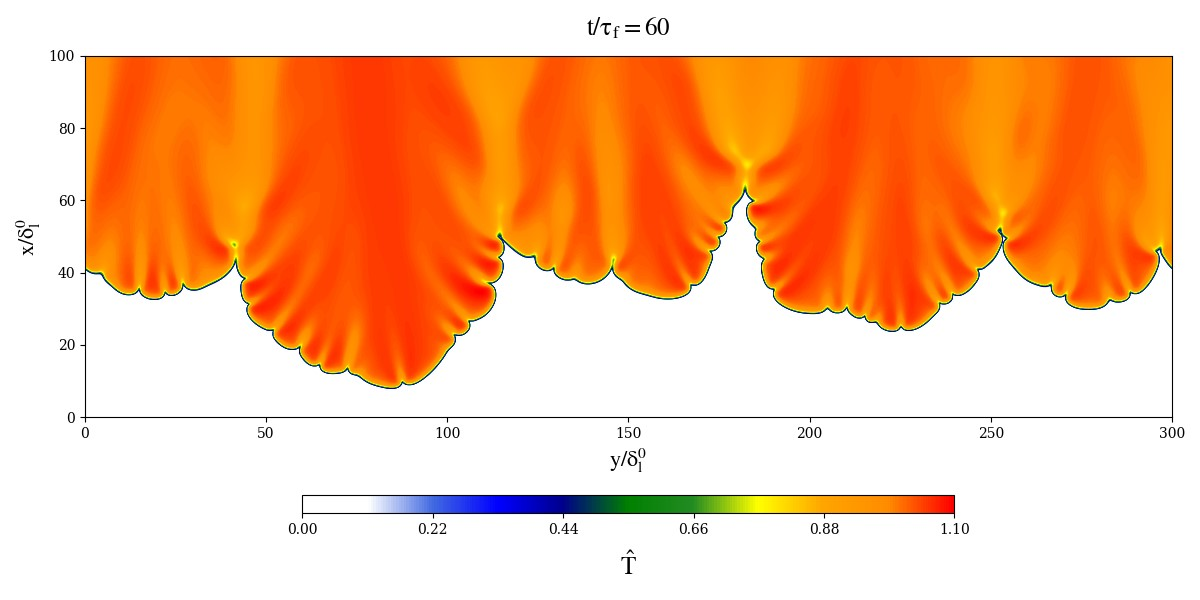
\includegraphics[angle=0, width=17cm]{figure.jpeg}
\caption{Non-dimensional temperature contour $\hat{T}$ at the flame front at $t/\tau_f = 60$. }
\label{Fig:1}
\end{figure}

A vertical space equivalent to a blank line must be inserted before and after each figure.

The legend for the data symbols as well as the labels for each curve should be included into the figure. Lettering should be large enough for ease reading. All units must be expressed in the S.I. (metric) system.

Color figures and high-quality photographs can be included in the manuscript. To reduce the file size and preserve the graphic resolution, figures must be saved into GIF (figures with less than 16 colors) or JPEG (for higher color density) files before being inserted in the manuscript.

Tables must be designated as either ``Tab.~\ref{Tab:1}'' in the middle of a sentence or ``Table~\ref{Tab:1}'' at the beginning of a sentence. Both the tables themselves and their titles must be centered in width. Table titles should be no longer than 3 lines. The font and size used in the tables must be similar to that used in the body of the text (both in size and style). Units must be given in the S.I. (metric) system. Any explanations should be at the foot of the tables, not in the tables themselves.

A vertical space equivalent to a blank line must be inserted before and after each table. The design of the table margins is up to you. An example can be found in Tab.~\ref{Tab:1}.

\begin{table}[!h]
\centering
\caption{Experimental results for flexural properties of CFRC-TWILL and CFRC-4HS composites. \protect\\Span/depth ratio = 35:1. Average results of 7 specimens.}
\label{Tab:1}
\begin{tabular}{l|c|c}
\hline
\textbf{Composite Properties} & \textbf{CFRC-TWILL} & \textbf{CFRC-4HS}\\
\hline
Flexural Strength\footnotesize{$^{(1)}$}, MPa & 209$\pm$ 10 & 180 $\pm$  15\\
Flexural Modulus\footnotesize{$^{(1)}$}, GPa & 57.0 $\pm$ 2.8 & 18.0 $\pm$  1.3\\
Mid-span deflection at the failure stress, mm & 2.15 $\pm$  1.90 & 6.40 $\pm$  0.25\\
\hline
\multicolumn{3}{l}{\footnotesize{$^{(1)}$ Measured at 25 $^{o}$C.}}
\end{tabular}
\end{table}

\section{ACKNOWLEDGEMENTS}

This optional section must be placed before the list of references. Authorship should be limited to those who made a significant contribution to the conception, design, execution, or interpretation of the reported study. If other individuals were involved in specific substantive aspects of the research project, they should be identified in this section. In addition, all sources of financial support for the project should be disclosed, as well as any potential situations that could be perceived as a conflict of interest.

The following text is an example:

We thank Prof. H. Simas for providing the lab floor and equipment used to make the prototype, and Dr. T. Hoeltgebaum of LAR - Prof. Raul Guenther Robotics Laboratory - UFSC for providing the raw data for their prototype. This work was funded by FAPESC under grant number xxxxxx/xxxx. The locomotion devices of the robot were kindly provided by TIF Robotics Ltd. 

\section{REFERENCES} 
\label{Sec:references}

The list of references must be inserted as a new section at the end of the manuscript. The first line of each reference must be left-justified. All other lines must be indented 0.5 cm from the left margin. All references listed in the reference list must have been mentioned in the text.

References must be listed in alphabetical order by the last name of the first author. See the following examples:

\bibliographystyle{abcm}
\renewcommand{\refname}{}
\bibliography{bibfile_template}

\section{RESPONSIBILITY NOTICE}
The following text, properly adapted to the number of authors, must be included in the last section of the paper:

The author(s) is (are) solely responsible for the printed material included in this paper.

\end{document}
